% Graphic for TeX using PGF
% Title: /home/kardelen/Insync/kardelenhatun@gmail.com/thesis_master/chapterzamk/images/cartesian.dia
% Creator: Dia v0.97.2
% CreationDate: Fri Dec 21 11:52:25 2012
% For: kardelen
% \usepackage{tikz}
% The following commands are not supported in PSTricks at present
% We define them conditionally, so when they are implemented,
% this pgf file will use them.
\ifx\du\undefined
  \newlength{\du}
\fi
\setlength{\du}{15\unitlength}
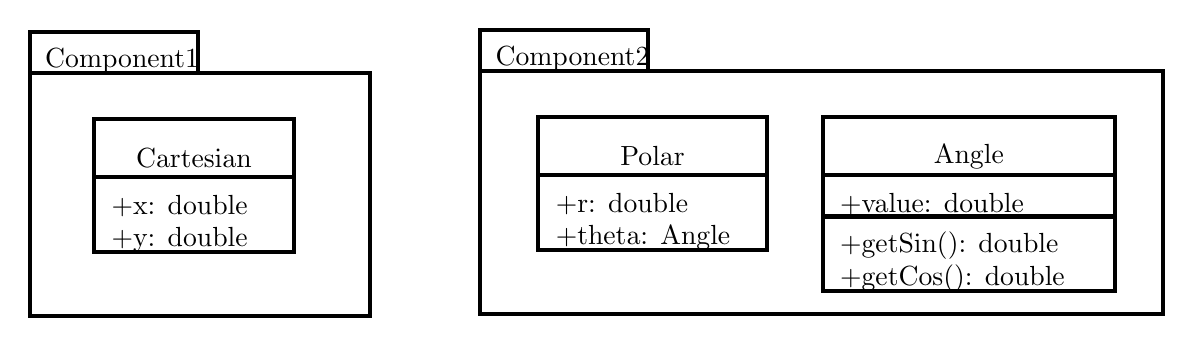
\begin{tikzpicture}
\pgftransformxscale{1.000000}
\pgftransformyscale{-1.000000}
\definecolor{dialinecolor}{rgb}{0.000000, 0.000000, 0.000000}
\pgfsetstrokecolor{dialinecolor}
\definecolor{dialinecolor}{rgb}{1.000000, 1.000000, 1.000000}
\pgfsetfillcolor{dialinecolor}
\pgfsetlinewidth{0.100000\du}
\pgfsetdash{}{0pt}
\definecolor{dialinecolor}{rgb}{1.000000, 1.000000, 1.000000}
\pgfsetfillcolor{dialinecolor}
\fill (5.700000\du,11.100000\du)--(5.700000\du,16.950000\du)--(13.900000\du,16.950000\du)--(13.900000\du,11.100000\du)--cycle;
\definecolor{dialinecolor}{rgb}{0.000000, 0.000000, 0.000000}
\pgfsetstrokecolor{dialinecolor}
\draw (5.700000\du,11.100000\du)--(5.700000\du,16.950000\du)--(13.900000\du,16.950000\du)--(13.900000\du,11.100000\du)--cycle;
\definecolor{dialinecolor}{rgb}{1.000000, 1.000000, 1.000000}
\pgfsetfillcolor{dialinecolor}
\fill (5.700000\du,10.100000\du)--(5.700000\du,11.100000\du)--(9.750000\du,11.100000\du)--(9.750000\du,10.100000\du)--cycle;
\definecolor{dialinecolor}{rgb}{0.000000, 0.000000, 0.000000}
\pgfsetstrokecolor{dialinecolor}
\draw (5.700000\du,10.100000\du)--(5.700000\du,11.100000\du)--(9.750000\du,11.100000\du)--(9.750000\du,10.100000\du)--cycle;
% setfont left to latex
\definecolor{dialinecolor}{rgb}{0.000000, 0.000000, 0.000000}
\pgfsetstrokecolor{dialinecolor}
\node[anchor=west] at (5.800000\du,10.800000\du){Component1};
\pgfsetlinewidth{0.100000\du}
\pgfsetdash{}{0pt}
\definecolor{dialinecolor}{rgb}{1.000000, 1.000000, 1.000000}
\pgfsetfillcolor{dialinecolor}
\fill (16.550000\du,11.050000\du)--(16.550000\du,16.900000\du)--(33.000000\du,16.900000\du)--(33.000000\du,11.050000\du)--cycle;
\definecolor{dialinecolor}{rgb}{0.000000, 0.000000, 0.000000}
\pgfsetstrokecolor{dialinecolor}
\draw (16.550000\du,11.050000\du)--(16.550000\du,16.900000\du)--(33.000000\du,16.900000\du)--(33.000000\du,11.050000\du)--cycle;
\definecolor{dialinecolor}{rgb}{1.000000, 1.000000, 1.000000}
\pgfsetfillcolor{dialinecolor}
\fill (16.550000\du,10.050000\du)--(16.550000\du,11.050000\du)--(20.600000\du,11.050000\du)--(20.600000\du,10.050000\du)--cycle;
\definecolor{dialinecolor}{rgb}{0.000000, 0.000000, 0.000000}
\pgfsetstrokecolor{dialinecolor}
\draw (16.550000\du,10.050000\du)--(16.550000\du,11.050000\du)--(20.600000\du,11.050000\du)--(20.600000\du,10.050000\du)--cycle;
% setfont left to latex
\definecolor{dialinecolor}{rgb}{0.000000, 0.000000, 0.000000}
\pgfsetstrokecolor{dialinecolor}
\node[anchor=west] at (16.650000\du,10.750000\du){Component2};
\pgfsetlinewidth{0.100000\du}
\pgfsetdash{}{0pt}
\definecolor{dialinecolor}{rgb}{1.000000, 1.000000, 1.000000}
\pgfsetfillcolor{dialinecolor}
\fill (17.950000\du,12.150000\du)--(17.950000\du,13.550000\du)--(23.455000\du,13.550000\du)--(23.455000\du,12.150000\du)--cycle;
\definecolor{dialinecolor}{rgb}{0.000000, 0.000000, 0.000000}
\pgfsetstrokecolor{dialinecolor}
\draw (17.950000\du,12.150000\du)--(17.950000\du,13.550000\du)--(23.455000\du,13.550000\du)--(23.455000\du,12.150000\du)--cycle;
% setfont left to latex
\definecolor{dialinecolor}{rgb}{0.000000, 0.000000, 0.000000}
\pgfsetstrokecolor{dialinecolor}
\node at (20.702500\du,13.100000\du){Polar};
\definecolor{dialinecolor}{rgb}{1.000000, 1.000000, 1.000000}
\pgfsetfillcolor{dialinecolor}
\fill (17.950000\du,13.550000\du)--(17.950000\du,15.350000\du)--(23.455000\du,15.350000\du)--(23.455000\du,13.550000\du)--cycle;
\definecolor{dialinecolor}{rgb}{0.000000, 0.000000, 0.000000}
\pgfsetstrokecolor{dialinecolor}
\draw (17.950000\du,13.550000\du)--(17.950000\du,15.350000\du)--(23.455000\du,15.350000\du)--(23.455000\du,13.550000\du)--cycle;
% setfont left to latex
\definecolor{dialinecolor}{rgb}{0.000000, 0.000000, 0.000000}
\pgfsetstrokecolor{dialinecolor}
\node[anchor=west] at (18.100000\du,14.250000\du){+r: double};
% setfont left to latex
\definecolor{dialinecolor}{rgb}{0.000000, 0.000000, 0.000000}
\pgfsetstrokecolor{dialinecolor}
\node[anchor=west] at (18.100000\du,15.050000\du){+theta: Angle};
\pgfsetlinewidth{0.100000\du}
\pgfsetdash{}{0pt}
\definecolor{dialinecolor}{rgb}{1.000000, 1.000000, 1.000000}
\pgfsetfillcolor{dialinecolor}
\fill (24.800000\du,12.150000\du)--(24.800000\du,13.550000\du)--(31.845000\du,13.550000\du)--(31.845000\du,12.150000\du)--cycle;
\definecolor{dialinecolor}{rgb}{0.000000, 0.000000, 0.000000}
\pgfsetstrokecolor{dialinecolor}
\draw (24.800000\du,12.150000\du)--(24.800000\du,13.550000\du)--(31.845000\du,13.550000\du)--(31.845000\du,12.150000\du)--cycle;
% setfont left to latex
\definecolor{dialinecolor}{rgb}{0.000000, 0.000000, 0.000000}
\pgfsetstrokecolor{dialinecolor}
\node at (28.322500\du,13.100000\du){Angle};
\definecolor{dialinecolor}{rgb}{1.000000, 1.000000, 1.000000}
\pgfsetfillcolor{dialinecolor}
\fill (24.800000\du,13.550000\du)--(24.800000\du,14.550000\du)--(31.845000\du,14.550000\du)--(31.845000\du,13.550000\du)--cycle;
\definecolor{dialinecolor}{rgb}{0.000000, 0.000000, 0.000000}
\pgfsetstrokecolor{dialinecolor}
\draw (24.800000\du,13.550000\du)--(24.800000\du,14.550000\du)--(31.845000\du,14.550000\du)--(31.845000\du,13.550000\du)--cycle;
% setfont left to latex
\definecolor{dialinecolor}{rgb}{0.000000, 0.000000, 0.000000}
\pgfsetstrokecolor{dialinecolor}
\node[anchor=west] at (24.950000\du,14.250000\du){+value: double};
\definecolor{dialinecolor}{rgb}{1.000000, 1.000000, 1.000000}
\pgfsetfillcolor{dialinecolor}
\fill (24.800000\du,14.550000\du)--(24.800000\du,16.350000\du)--(31.845000\du,16.350000\du)--(31.845000\du,14.550000\du)--cycle;
\definecolor{dialinecolor}{rgb}{0.000000, 0.000000, 0.000000}
\pgfsetstrokecolor{dialinecolor}
\draw (24.800000\du,14.550000\du)--(24.800000\du,16.350000\du)--(31.845000\du,16.350000\du)--(31.845000\du,14.550000\du)--cycle;
% setfont left to latex
\definecolor{dialinecolor}{rgb}{0.000000, 0.000000, 0.000000}
\pgfsetstrokecolor{dialinecolor}
\node[anchor=west] at (24.950000\du,15.250000\du){+getSin(): double};
% setfont left to latex
\definecolor{dialinecolor}{rgb}{0.000000, 0.000000, 0.000000}
\pgfsetstrokecolor{dialinecolor}
\node[anchor=west] at (24.950000\du,16.050000\du){+getCos(): double};
\pgfsetlinewidth{0.100000\du}
\pgfsetdash{}{0pt}
\definecolor{dialinecolor}{rgb}{1.000000, 1.000000, 1.000000}
\pgfsetfillcolor{dialinecolor}
\fill (7.250000\du,12.200000\du)--(7.250000\du,13.600000\du)--(12.057500\du,13.600000\du)--(12.057500\du,12.200000\du)--cycle;
\definecolor{dialinecolor}{rgb}{0.000000, 0.000000, 0.000000}
\pgfsetstrokecolor{dialinecolor}
\draw (7.250000\du,12.200000\du)--(7.250000\du,13.600000\du)--(12.057500\du,13.600000\du)--(12.057500\du,12.200000\du)--cycle;
% setfont left to latex
\definecolor{dialinecolor}{rgb}{0.000000, 0.000000, 0.000000}
\pgfsetstrokecolor{dialinecolor}
\node at (9.653750\du,13.150000\du){Cartesian};
\definecolor{dialinecolor}{rgb}{1.000000, 1.000000, 1.000000}
\pgfsetfillcolor{dialinecolor}
\fill (7.250000\du,13.600000\du)--(7.250000\du,15.400000\du)--(12.057500\du,15.400000\du)--(12.057500\du,13.600000\du)--cycle;
\definecolor{dialinecolor}{rgb}{0.000000, 0.000000, 0.000000}
\pgfsetstrokecolor{dialinecolor}
\draw (7.250000\du,13.600000\du)--(7.250000\du,15.400000\du)--(12.057500\du,15.400000\du)--(12.057500\du,13.600000\du)--cycle;
% setfont left to latex
\definecolor{dialinecolor}{rgb}{0.000000, 0.000000, 0.000000}
\pgfsetstrokecolor{dialinecolor}
\node[anchor=west] at (7.400000\du,14.300000\du){+x: double};
% setfont left to latex
\definecolor{dialinecolor}{rgb}{0.000000, 0.000000, 0.000000}
\pgfsetstrokecolor{dialinecolor}
\node[anchor=west] at (7.400000\du,15.100000\du){+y: double};
\end{tikzpicture}
